\documentclass{school-22.211-notes}
\date{February 27, 2012}

\begin{document}
\maketitle

\clearpage
\topic{Resonance Models}
Reference: Alain Hebert's Applied Reactor Physics (p.199-202), Duderstadt's p.343-347. 

Recall the assumptions we made for slowing down equation: 
\begin{itemize}
\item Steady state.
\item Infinite medium: there is no spacial dependency. 
\item No external source. 
\item S-wave elastic scattering (that is isotropic in COM frame) for light nuclides, 
    \eqn{ \Sigma_s (E' \to E) &= \frac{\Sigma_s(E')}{(1-\alpha)E'} &\mbox{for } E < E' < \frac{E}{\alpha} }
  where $\alpha = (A-1/A+1)^2$.
\end{itemize}
For resonance models, we have to take into account inelastic scattering for heavy isotopes by introducing the 0-th and 1-st Legrendre modes. 


%%%% 12 fall 
Recall the slowing down equation for resonance region $[1\eV, 0.1 \MeV]$, 
\begin{align}
\Sigma_t (u) \Phi(u) &= \int_{u-\epsilon}^u \frac{1}{1 - \alpha} e^{-(u-u')} \Sigma_s (u') \Phi(u') \du' \label{resonance-sl-d-eqn} \\
(\Sigma_{t1}(u) + \Sigma_{t0} (u)) \Phi(u) &= \int_{u - \epsilon_0}^u \frac{1}{1 - \alpha_0} e^{-(u-u')} \Sigma_{s0}(u') \Phi(u') \du' + \int_{u-\epsilon_1}^u \frac{1}{1 - \alpha_1} e^{-(u-u')} \Sigma_{s1} (u') \Phi(u') \du'  
\end{align}

Next we manipulate the above equations:
\begin{itemize}
\item We facterize $\Phi(u) = \phi(u) \Psi(u)$, where $\phi(u)$ is the fine structure/self-shielding factor that models the resonances, $\Psi(u)$ is the flux outside the resonance (Hebert calls it `macroscopic flux', and it represents the asymptotic behavior of flux between resonances). 

\item Because of the 1/E flux between resonances (or constant in lethargy) $\Phi(u) = \frac{q(u)}{\xi \Sigma_s}$, we write the RHS of Eq.~\ref{resonance-sl-d-eqn} as $R \Phi(u)$. $R$ has two components. We do not know what $R_0$ is yet,
\eqn{  R_0 \Phi(u) &= R_0 \phi(u) \Psi(u) = \int_{u-\epsilon_0}^u \frac{1}{1-\alpha_0} e^{-(u-u')} \Sigma_{s0}(u') \phi(u') \Psi(u') \du'  }
But for the 1st order, we apply the 1/E flux between resonance part and get rid of the $\phi(u)$ term, 
\eqn{ R_1 \Phi(u) &= \Sigma_{t1} \Psi(u)  }

\item Then we can write (omitting every term's $u$ dependency), then cancel out $\Psi$ on both sides, 
\begin{align}
 (\Sigma_{t1} + \Sigma_{t0}) \Psi \phi &= R_0 \Psi \phi +  \Sigma_{t1} \Psi    \\
R_0 \phi + \Sigma_{t1} &= (\Sigma_{t1}  + \Sigma_{t0} ) \phi 
\end{align}

\item If we divide by $N_0$ (the resonance nuclide number density), we get 
\eqn{ r_0 \phi + \sigma_d &= (\sigma_d + \sigma_{to}) \phi }
\end{itemize}


There are a couple of ways to approximate $r_0 \phi(u)$. 

%%%% 12 fall end

\begin{enumerate}
\item Wide resonance assumes that the resonances are so large that we can assume the reaction rate (for the fine structure) is constant. 
\eqn{ r_0 \phi(u) &= \int_{u-\epsilon_0}^u \frac{1}{1-\alpha_0} e^{-(u-u')} \overbrace{ \sigma_{so} (u') \phi(u')}^{\mathrm{constant}} \du' = \sigma_{s0} (u) \phi(u)  }
Then we arrive at, 
\eqn{ \phi_{WR} (u) &= \frac{\sigma_d}{\sigma_{to} (u) - \sigma_{s0} (u) + \sigma_d}  }
%


Connecting with other properties:
\begin{align}
\phi_{WR} (u) &= \frac{\sigma_d}{\sigma_{a}^R (u) +  \sigma_d } \\
\RIeff^{\gamma} &= \int \sigma_{\gamma}^R (u) \phi_{WR} (u) \du \\
&= \int \sigma_{\gamma}^R (u) \frac{\sigma_d}{\sigma_a^R(u) + \sigma_d} \du \\
&= \Ln{\frac{E_2}{E_1}} \frac{ \int \sigma_{\gamma}^R (E) \frac{\sigma_d}{\sigma_{a}^R(E) + \sigma_d} \frac{1}{E} \dE}{ \int \frac{\sigma_d}{\sigma_{a}^R(E) + \sigma_d} \frac{1}{E} \dE}
\end{align}
Notice wide resonance approximation $\RI_{\eff}$ only depends on cross sections: $\sigma_d$ is assumed to be based on material composition of the reactor, and $\sigma_r(E)$ are from libraries. There is no need for flux spectrum. 

The wide resonance approximation says that we ignore scattering of U238 because its width is large compared with the approximately 1\% energy it can lose upon scattering. To improve this approximation, sometimes people use the potential scattering of 11.39 barns. 

Wide resonance approximations match direct MC results near infinite dilution. 




\item Narrow resonance approximations assume resonance is very narrow, thus cross section remains the same, thus $\Phi(E) \propto 1/E, \Phi(u) = $constant. Thus we can write, 
\eqn{ r_0 \phi(u) = \int_{u-\epsilon_0}^u \frac{1}{1- \alpha_0} e^{-(u-u')} \sigma_{s0}(u') \Phi(u') \du' }
where $\Phi(u') = 1, \sigma_{s0} (u')\approx \sigma_{po}$ potential scattering, also 
\eqn{ \int_{u-\epsilon}^u \frac{1}{1-\alpha_0} e^{-(u-u')} \du' = 1} 
Thus narrow resonance approximation leads to, 
\eqn{ r_0 \phi(u) = \sigma_{po}}
That is, 
\eqn{ \sigma_{po} + \sigma_d &= (\sigma_d + \sigma_{t0} (u)) \phi_{NR} (u) & \phi_{NR} (u) &= \frac{\sigma_{po} + \sigma_d}{\sigma_d + \sigma_{to} (u) } }




Narrow resonance approximations assume the opposite of the wide resonance approximation, that the neutron is going to be out of the resonance upon one scattering. This approximation is good for higher energy. For instance, at 100 keV, scattering lose 1 keV, which is larger than the 25 eV spacing of \ce{^{238}U}. 
\begin{align}
\phi_{NR} (u) &= \frac{\sigma_{pot}^R + \sigma_d}{\sigma_{a}^R + \sigma_{pot}^R + \sigma_d } \\
\RIeff^{\gamma} &= \int \sigma_{\gamma}^R (u) \phi_{NR} (u) \du \\
&= \int \sigma_{\gamma}^R (u) \frac{\sigma_{pot}^R + \sigma_d}{\sigma_a^R(u) + \sigma_{pot}^R + \sigma_d} \du \\
&= \Ln{\frac{E_2}{E_1}} \frac{ \int \sigma_{\gamma}^R (E) \frac{\sigma_{pot}^R + \sigma_d}{\sigma_{a}^R(E) + \sigma_{pot}^R + \sigma_d} \frac{1}{E} \dE}{ \int \frac{\sigma_{pot}^R + \sigma_d}{\sigma_{a}^R(E) + \sigma_{pot}^R + \sigma_d} \frac{1}{E} \dE}
\end{align}
However, the results on the slides come out to be that narrow resonance approximation is not really any better than the wide resonance approximation at higher energy, so there must be some other physics going on. 

Narrow resonance approximation is good at high energies. For fast reactor applications for instance narrow resonance is used a lot. 


\item Narrow vs. Wide Resonance Approximations\label{narrow-wide-compr}. 
Wide resonance approximation agrees pretty well with MC results without U238 scattering; narrow resonance approximation agrees alright with the MC results with U238 scattering. Notice adding in scattering would change the low dilution factor results. See Figure~\ref{wide-vs-narrow}.

Compare with MC results using real U238 and U235 xs data, the real results fall between the wide and the narrow approximations for the high dilution factor; but for the low dilution factor, that is, when there are lots of resonance material (uranium), the physics gets complicated: 
\begin{itemize}
\item Non 1/E slowing down sources;
\item Non constant moderator xs;
\item Resonance scattering alters sources;
\item We may have multiple resonance in each RI group; that is, each of our RI does not include a single resonance anymore;
\item Resonance interference between \ce{^{235}U} and \ce{^{238}U}; eg: \ce{^{238}U}'s resonance spacing is 25 eV, whereas \ce{^{235}U}'s resonance spacing is 5 eV, that is, for each \ce{^{238}U} resonance, there are multiple \ce{^{235}U} resonances on top of it. 
\end{itemize}
\begin{figure}
  \centering
  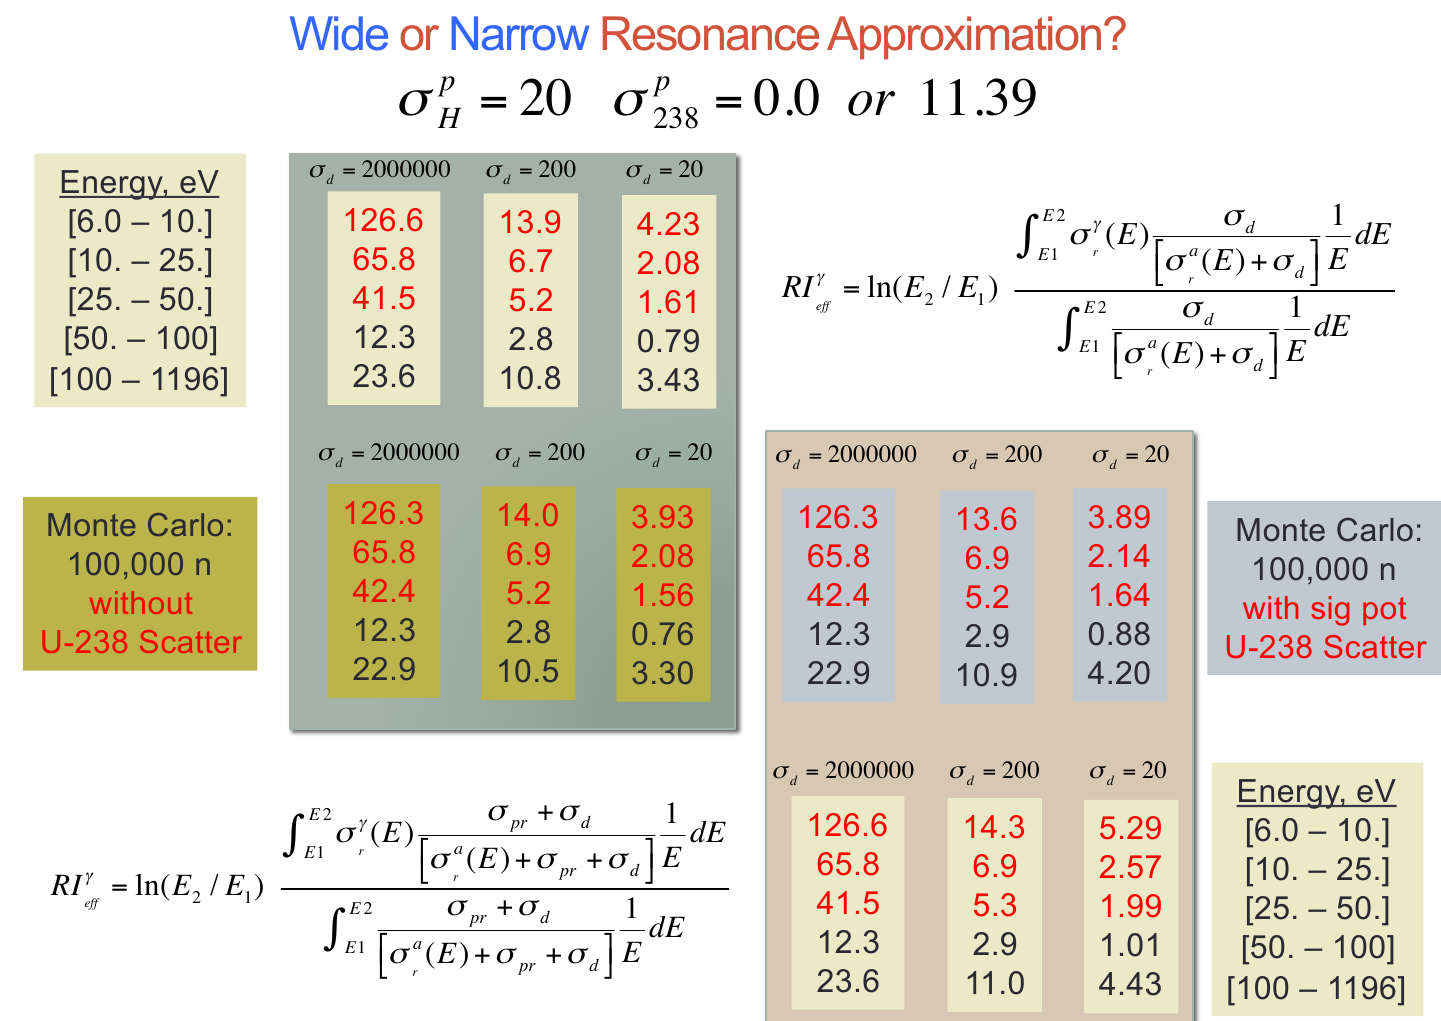
\includegraphics[width=4in]{images/r-m/narrow-vs-wide-resonance.png}
  \caption{Comparison Of Wide and Narrow Resonance Approximation} \label{wide-vs-narrow}
\end{figure}


% 12fall
\item Goldstein-Cohen Model: since isotopes are going to be somewhere between the two extremes, we consider a linear combination of $\psi_{NR}, \psi_{WR}$, 
\eqn{ \phi_{GC} (u) = \frac{\lambda_g \sigma_{po} + \sigma_d}{\sigma_{to}(u) - (1-\lambda_g) \sigma_{so}(u) + \sigma_d } }
where $\lambda_g$ depends on isotope and energy band. When $\lambda_g = 1$ we get the $\psi_{NR}$, $\lambda_g = 0$ we get the $\psi_{WR}$. 

Alternatively, we can discretize our energy group very finely, then we would not need any resonance models. 
\end{enumerate}




How does a prudction tool uses resonance parameters?

\textbf{Normal procedure} for generating multi-group xs in a code like NJOY includes:
\begin{enumerate}
\item Use code to Doppler broaden cross sections for each resonance isotope for range of temperatures (eg, 300, 600, 900, 2000K); 
\item Use code to apply the narrow or wide resonance models for a range of dilution xs (eg, 20000, 2000, 200, 20 barns); 
\item Edit RIs or multi-group xs for your desired energy structure; 
\item Build tables of xs vs. dilution xs and temperature;
\item For downstream computations, interpolate for the dilution cross section and temperature of each material in the simulation to obtain accurate multigroup cross sections for that specific applications. 
\end{enumerate}

\textbf{A better procedure} for generating multi-group cross sections includes:
\begin{enumerate}
\item Same;
\item Use code to solve real neutron slowing down problem for a range of dilution cross sections (eg, 20000, 2000, 200, 20 barns);
\item Consider including a mix of resonance absorbers to make the spectrum as appropriate to the desired application as possible;
\item Same;
\item Same;
\item Same.
\end{enumerate}

\textbf{For downstream applications} that require cross section data, for each resonance group,
\begin{enumerate}
\item For each composition, evaluate the material temperature and isotopic densities. 
\item Evaluate Dancoff from pin diameter, lattice pitch, etc. 
\item Compute the escape cross section for each resonance absorber.
\item Evaluate group cross section (or RI) using Dancoff, potential and escape cross sections by interpolating cross section (or RI) tables at appropriate temperatures. 
\end{enumerate}

For real application, it is rarely possible to just use someone else's cross section table; we almost certainly need to generate xs suitable for our application. 



%%%%%%%% 12 Fall 
\clearpage
\topic{Examples Using Resonance Models}
Recall:
\begin{itemize}
\item Flux facterization $\Phi(u) = \phi(u) \Psi(u)$ where $\phi$ is the fine structure function, $\Psi(u)$ is the flux outside the resonance. 
\item Dilution cross section: 
  \eqn{ \sigma_d = \frac{\Sum_{\mathrm{moderator}} N_m \sigma_m}{N_r} }
\item Narrow resonance approximation\footnote{the only energy/lethargy dependent term on the RHS should be $\sigma_{to}(u)$.}:
  \eqn{ \phi_{NR} (u) = \frac{\sigma_{po} + \sigma_d}{\sigma_d + \sigma_{to}(u)} }
\end{itemize}

There are two possibilites in using NR approximation to calculate the condensed cross section depends on the number of resonant isotopes: 
\begin{enumerate}
\item One resonant isotope. Assume we have \ce{H_2 O} and \ce{^{235} U}. 
\begin{align}
\sigma_d &= \frac{N_H \sigma_H + N_O \sigma_O}{N_U} 
\end{align}
We evaluate $\phi$ using narrow resonance approximation: 
  \eqn{ \phi_{NR} (u) = \frac{\sigma_{po} + \sigma_d}{\sigma_d + \sigma_{to}(u)} }
Then the flux-weighted resonant material cross section is,
\eqn{ \sigma_{U,g} = \frac{\int \sigma_{U}(u) \psi(u) \du}{\int \psi(u) \du} }

\item Multiple resonant isotopes. Assume we have \ce{H_2 O}, \ce{^{235}U}, and \ce{^{238} U}. 

  \textbf{Solution 1:}
  \begin{enumerate}
  \item Assume \ce{^{235} U} is the only resonant isotope, then we solve an energy independent $\sigma_d$ by 
    \eqn{ \sigma_d = \frac{N_{238} \bar{\sigma}_{238} + N_H \sigma_H + N_O \sigma_O}{N_{235} } }
    Then we solve for $\psi(u)$:
      \eqn{ \phi_{NR} (u) = \frac{\sigma_{po,235} + \sigma_d}{\sigma_d + \sigma_{to,235}(u)} \label{NR-flux-eqn}  }
    Then calculate the collapsed $\bar{\sigma}_{235}$:
    \eqn{ \bar{\sigma}_{235} = \frac{\int \sigma_{235} (u) \phi(u) \du}{\int \phi(u) \du}  \label{flux-collapse-235}  }
  \item Assume \ce{^{238} U} is the only resonant isotope. 
    \eqn{ \sigma_d = \frac{N_{235} \bar{\sigma}_{235} + N_H \sigma_H + N_O \sigma_O}{N_{238} } }
    Then we solve for $\psi(u)$:
      \eqn{ \phi_{NR} (u) = \frac{\sigma_{po,238} + \sigma_d}{\sigma_d + \sigma_{to,238}(u)} }
    Then calculate the collapsed $\bar{\sigma}_{238}$:
    \eqn{ \bar{\sigma}_{238} = \frac{\int \sigma_{238} (u) \phi(u) \du}{\int \phi(u) \du}   }
  \end{enumerate}
  Then we feed $\bar{\sigma}_{238}$ back into step 1 and repeat the process until $\bar{\sigma}_{235}, \bar{\sigma}_{238}$ converge, which happen fairly fast with a simple resonance. 


\textbf{Solution 2 (Nate/Gene)}: 

In Eq.~\ref{flux-collapse-235}, $\phi(u)$ shows up in both the top and the bottom of the equation, so if we scale $\phi(u)$ by any non-energy dependent term as they would just cancel out, the solution would not change. Recall $\phi(u)$ as in Eq.~\ref{NR-flux-eqn}, the top $\sigma_{po,r} + \sigma_d$ is energy-independent, and $N_r$ is energy-independent as well, that is, 
\eqn{ \phi_{NR} (u) = \frac{\sigma_{po,r} + \sigma_d}{\sigma_d + \sigma_{to,r}(u)} \to \frac{1}{\sigma_d + \sigma_{to,r}(u)} \to  \frac{1}{N_r \sigma_d + N_r \sigma_{to,r}(u)} \to \frac{1}{\Sum_{\mathrm{moderators}} N_m \sigma_m + N_r \sigma_{to,r}(u)} }
Then the total flux is fine structure times a $1/E$ dependency, 
\eqn{ \Phi (E) = \frac{1}{E \left[ \Sum_{\mathrm{moderators}} N_m \sigma_m + N_r \sigma_{to,r}(E)\right]} }
Then we don't have to compute $\sigma_d$ anymore. For each resonant isotope, the three steps becomes two steps: calculating $\Phi$ using last step's condensed cross section, and update this step's condensed cross section with $\Phi$-collapsed cross section. 

So effectively narrow resonance suggest, 
\eqn{ \Phi (E)  = \frac{1}{E \Sigma_t (E)} }

\end{enumerate}













\end{document}
